%%%%%%%%%%%%%%%%%%%%%%%%%%%%%%%%%%%%%%%%%%%%%%%%%%%%%%%%%%%%%%%%%%%%
% Diskussion und Ausblick
%%%%%%%%%%%%%%%%%%%%%%%%%%%%%%%%%%%%%%%%%%%%%%%%%%%%%%%%%%%%%%%%%%%%

\chapter{React - Theorie und Evaluation}
  \label{Evalution React}

\section{Motivation}
React wurde 2013 von Facebook entwickelt. Seine Entstehung ist direkt verknüpft mit den Problemen von JavaScript, die speziell bei großen Anwendungen auftreten. Das von JavaScript verwendete DOM ist bei oftmaligen Zustandsänderungen langsam und ineffizient. Durch den Aufbau des DOM muss dieses auch bei kleinen Änderungen in Gänze neu geladen werden. Es gilt außerdem allgemein als fehleranfällig, unnötig kompliziert und ist für die Webentwicklung nicht sehr gut geeignet. \cite{2}\\
Hinzu kommt, dass JavaScript-Objekte nicht funktional sind, das heißt ihr Zustand ist nicht nur vom Input und darauf ausgeführten Funktionen abhängig. Stattdessen teilen sich Objekte oftmals Zustände und verändern sich so mitunter gegenseitig. Daher war Frontendcode vor React oft unverständlich und schwer wartbar. \cite{2}\\
Das Ziel der Entwicklung Reacts war es deswegen weniger komplexen und gut lesbaren Code zu ermöglichen, der Zustände persistent und effizient verwaltet \cite{3}. Die sonst oft in der Webentwicklung verwendeten Templates sollten ersetzt werden. Stattdessen sollte eine Lösung die mehr Flexibilität bietet und es gleichzeitig durch kompaktere Architektur erleichtert Applikationen auszuweiten eingeführt werden \cite{1}.
\section{Architektur}
Im Vergleich zu den bis dato gängigen JavaScript Frameworks und JavaScript selbst, weist React einige Besonderheiten in seiner Architektur auf. Die wichtigsten dieser Besonderheiten werden hier im Folgenden aufgeführt und diskutiert. Es gibt noch einige weitere Eigenheiten Reacts, doch diese vier sind die ausschlaggebenden Merkmale für dessen Erfolg und stehen deshalb im Fokus dieser Evaluation.
\subsection{Virtual DOM}
In der Webentwicklung hat die Manipulation des Document Object Model (DOM) eine ausschlaggebende Rolle inne. Mit ihr kann der Elementbaum einer Webseite ausgelesen, verändert und erweitert werden. Wie oben erwähnt ist das JavaScript DOM problematisch.\\
React löst dieses Problem mittels dem sogenannten Virtual DOM, welche ein entsprechendes virtuelles Model des eigentlichen DOMs ist \cite{4}. Jedes DOM-Objekt wird darin über ein ähnliches oder vereinfachtes virtuelles Objekt dargestellt. Obwohl es in seinen Eigenschaften dem DOM stark ähnelt, kann das virtuelle DOM keine direkten Änderungen am Elementbaum durchführen. Stattdessen wird seine erheblich bessere Performanz als Änderungsbuffer benutzt. Wird ein React Komponent (siehe 2.3) gerendert, so wird ein Snapshot des aktuellen Zustands gemacht und alle virtuellen DOM-Objekte werden aktualisiert. Dieser Prozess ist weitaus schneller als das Aktualisieren des eigenlichen DOM, da keine tatsächlich angezeigten Elemente verändert werden. Dabei beeinflusst er die Performanz des restlichen Systems nicht. Nachdem so alle virtuellen DOM-Objekte aktualisiert wurden, werden diese mittels dem sogennanten 'Diffing' mit dem Snapshot verglichen. Lediglich der Zustand der Objekte der sich zwischen diesen Schritten verändert hat, wird vom virtuellen DOM in das DOM übernommen \cite{3}. In Abbildung 2.1 ist dieser Prozess in einem Schaubild dargestellt.\\
\begin{figure}[H]
     \centerline{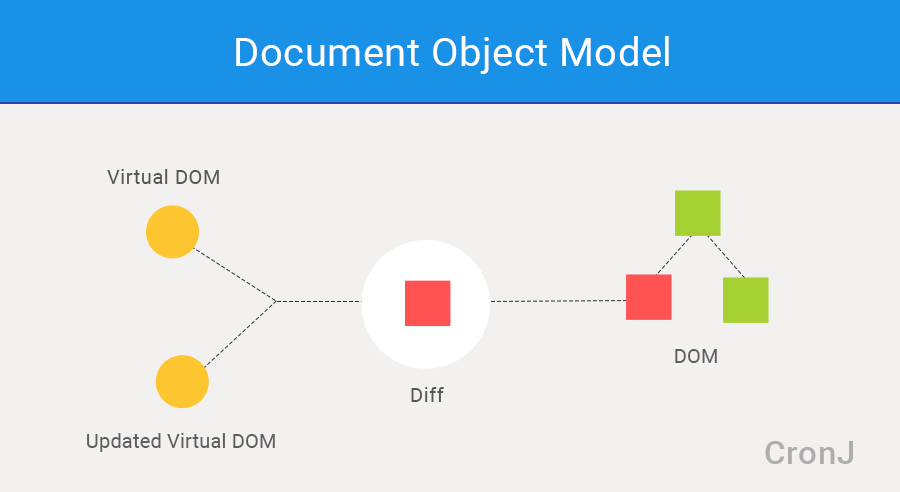
\includegraphics[width=14cm]{../Abbildungen/virtualDom.png}}
  \caption{React Virtual DOM \cite{Abb2.1}}
  \label{React Virtual DOM}
\end{figure}
\noindent Resultat ist eine erheblich schnellere, effizientere und performantere DOM-Manipulation als frühere Lösungen. Das Virtual DOM kann fraglos als einer der Hauptgründe für Reacts Beliebtheit bezeichnet werden.
\subsection{Komponenten}
Komponenten sind die wichtigsten Bausteine einer React Anwendung. Sie sind vergleichbar mit JavaScript Klassen und Funktionen. Mit sogenannten Props (Properties) als Input liefern Komponenten React-Elemente an die View. So legen sie das Aussehen eines Teils der Benutzeroberfläche fest, deren Gesamtheit aus vielen verschachtelten Komponenten besteht. Ein Beispiel einer simplen 'Hello World'-Komponente in React ist in Abbildung 2.2 abgebildet.
\begin{figure}[H]
     \centerline{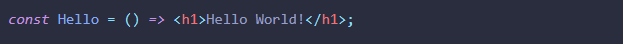
\includegraphics[width=12cm]{../Abbildungen/compHello.png}}
  \caption{Hello World Komponente \cite{eig}}
  \label{Hello World Komponente}
\end{figure}
Komponenten sind wiederverwendbar und veränderbar. Durch die Implementierung von Komponenten besteht die Benutzeroberfläche in React aus diesen vielen kleinen Elementen des gleichen Typs und ist dadurch leicht anzupassen, nachzuvollziehen und zu testen. Sind Änderungen an einer bestimmten Komponente nötig, so kann direkt auf diese zugegriffen und ihr Inhalt verändert werden. Am Beispiel in Abbildung 2.3 die dem React-Lehrbuch 'Learning React' entnommen ist, ist dies gut zu erkennen. Hier markiert jeder der rechteckigen Ränder eine Komponente. Wäre es nötig die Zubereitung des 'Curried Egg Salad' zu ändern, ist dies problemlos möglich da es eine eigene Komponente ist. So ist kein Zugriff auf andere Komponenten nötig und es wird eine versehentliche Änderung dieser ausgeschlossen.\\
\begin{figure}[H]
     \centerline{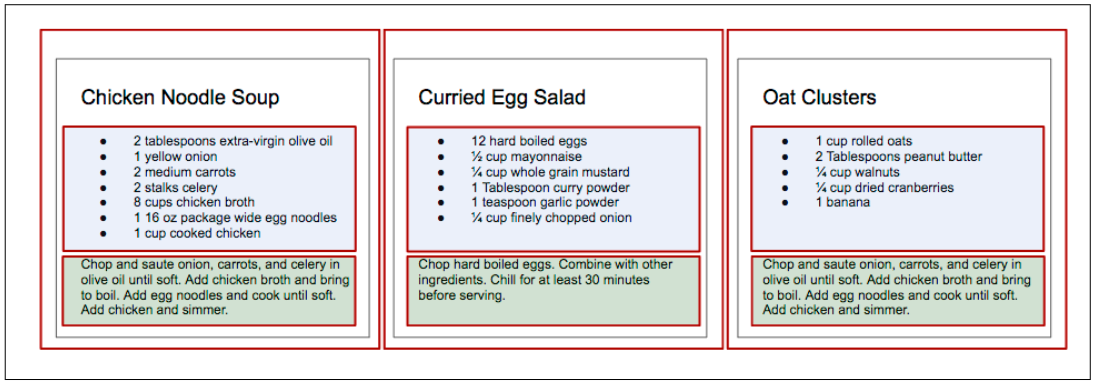
\includegraphics[width=12cm]{../Abbildungen/compContainer.png}}
  \caption{Hello World Komponente \cite{6}}
  \label{Hello World Komponente}
\end{figure}
\clearpage
\subsection{Unidirektionaler Datenfluss}
Anders als viele der beliebten Frameworks verwendet React keinen bidirektionalen Datenfluss. Ebenso erstellt es in dem bekannten Model-View-Controller Konzept nur die View-Komponente und überlässt dem Entwickler die Wahl, ob und welche weiteren Komponenten verwendet werden \cite{5}. In einem bidirektionalen Datenfluss sind Model und View in direktem, gegenseitigem Austausch \cite{5}. In diesem Austausch lösen Änderungen an einer Seite entsprechende Änderungen auf der anderen Seite aus. Diese gängige Lösung wird in den meisten Fällen gute Leistungen und Ergebnisse erzielen. Jedoch können unvorhersehbaren Datenflüsse auftreten, eben weil sowohl Model als auch View Einfluss auf den Zustand der Anwendung haben. Es kann so zu nicht beabsichtigten Änderungen in nicht bearbeiteten Model-Bereichen und zu Kettenreaktionen von Updates kommen.\\
In React können Daten stattdessen nur in eine Richtung gegeben und verarbeitet werden, React ist also unidirektional. So wird ein Jonglieren der Zustände vermieden. \\
\begin{figure}[H]
     \centerline{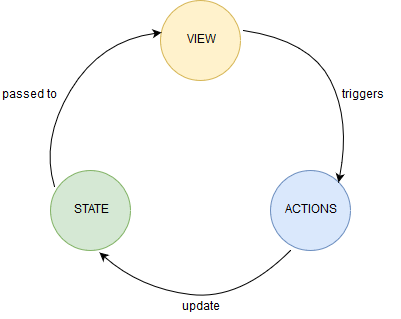
\includegraphics[width=12cm]{../Abbildungen/dataflow.png}}
  \caption{Unidirektionaler Datenfluss in React \cite{eig}}
  \label{Unidirektionaler Datenfluss in React}
\end{figure}
\clearpage \noindent In Abbildung 2.4 ist zu sehen, wie die Daten hier in einem Kreislauf durch Zustand, View und Aktionen fließen. Der Anwendungszustand, der die Zustände der Komponenten beinhaltet, wird an die View und ihre Child-Komponenten weitergegeben. In dieser werden Aktionen getriggered, beispielsweise durch den Nutzer, welche den Zustand verändern können. \\
Wie in Punkt 2.1 erwähnt, konnte es vor React oftmals schwierig sein den Datenfluss in einer Anwendung nachzuverfolgen. Der unidirektionale Datenfluss Reacts schafft hier eine größere Nachvollziehbarkeit und begünstigt so Analyse und Fehlersuche. \\
\subsection{JSX}
JSX ist eine Syntax-Erweiterung zu JavaScript die für React empfehlenswert ist, da sie durch ihre Ähnlichkeit mit HTML-Syntax leicht zu lesen und zu verwenden ist \cite{5}. Der Typ eines Elements wird wie in HTML in einem öffnenden Tag festgelegt. Zwischen diesem öffnendem und dem nachfolgenden schließendem Tag können die Kinder des Elements hinzugefügt werden. In Abbildung 2.5 ist als Beispiel eine ungeordnete Liste in JSX dargestellt.
\begin{figure}[!thb]
     \centerline{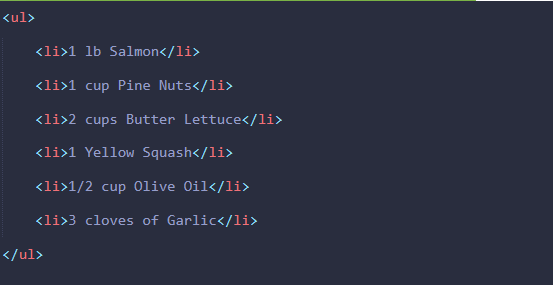
\includegraphics[width=12cm]{../Abbildungen/jsxList.png}}
  \caption{Ungeordnete Liste in JSX \cite{eig}}
  \label{Ungeordnete Liste in JSX}
\end{figure}
In JSX werden JavaScript-Ausdrücke in geschweifte Klammern gestellt. Die Anzeige des Titel-Felds eines Elements wäre beispielsweise wie in Abbildung 2.6 umzusetzen.\\ 
\begin{figure}[H]
     \centerline{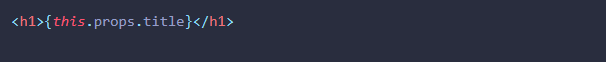
\includegraphics[width=12cm]{../Abbildungen/jsxExpression.png}}
  \caption{JavaScript in JSX \cite{eig}}
  \label{JavaScript in JSX}
  \centerline{}
     \centerline{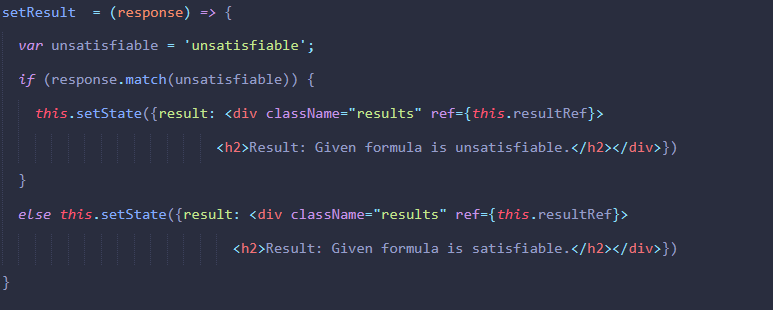
\includegraphics[width=12cm]{../Abbildungen/jsxSetResult.png}}
  \caption{Funktion setResult in JSX \cite{eig}}
  \label{Funktion setResult in JSX}
\end{figure}
\noindent Die Ausdrücke werden als vollwertiges Skript ausgeführt, es ist daher auch möglich vorher definierte Funktionen und vorimplementierte JavaScript Operationen an dieser Stelle zu verwenden. Da JSX eine Erweiterung zu JavaScript ist, kann in derartigen Funktionen auch JSX-Syntax verwendet werden. Wie in Abbildung 2.7 gezeigt, könnte beispielsweise eine Funktion setResult erstellt werden, die einen erhaltenen String untersucht und abhängig von dessen Inhalt zwei unterschiedliche JSX-Sequenzen ausgibt. \\
JSX bietet einige Vorteile gegenüber dem üblichen JavaScript. Da JSX-Code während er zu JavaScript kompiliert automatisch optimiert wird, sind Anwendungen in JSX mindestens gleich schnell wie equivalente Anwendungen in JavaScript. Dieses Kompilieren fängt außerdem Fehler ab und erhöht so die Qualität der Anwendung. Diese Wirkung wird noch verstärkt durch die zusätzlichen Debugging Möglichkeiten die JSX auf Compiler Level bietet. Dank der Syntax die HTML und JavaScript vereint, ist JSX sehr leicht zugänglich und benötigt wenig Einarbeitungszeit. \\
Als interpretierte Programmiersprache wird JavaScript üblicherweise ohne vorherigen Kompilierschritt vom Browser gelesen und interpretiert. Da Browser aber JSX nicht erkennen, ist Kompilieren hier notwendig. Dieser Prozess wird auch Transpiling genannt. Üblich ist hier die Nutzung des Babel-Projekts, welches auch von den großen React-Nutzern Facebook, PayPal, Netflix und AirBnB genutzt wird und welches schon über einen kurzen Import genutzt werden kann \cite{6}. Da die Verwendung von Toolchains (siehe Punkt 3.1.2) diese Konfiguration automatisch übernimmt, ist es jedoch sehr selten nötig dies selbst zu tun.\\
\section{Stärken}
Wie in den Passagen oben zu sehen, gibt es gute Gründe warum React so schnell so beliebt wurde. Als Bibliothek für JavaScript ist React ein Teil der beliebtesten Programmiersprache für Webseiten der Welt und verbessert diese an den nötigen Stellen. Reacts virtuelle DOM ist schnell, effizient und dynamisch und so der JavaScript DOM überlegen. Der unidirektionale Datenfluss bietet als neuer Ansatz ebenso einige Vorteile gegenüber dem bidirektionalen Fluss anderer Frameworks. Durch diese Besonderheiten seiner Architektur ist es auch für große Webanwendungen gut geeignet. Besonders die Fehleranfälligkeit und Unsicherheit JavaScripts konnte verbessert werden \cite{6}.\\
Mit der JSX-Syntax und der Nähe zur funktionalen Programmierung sind React Anwendungen intuitiv, übersichtlich, gut testbar und bieten eine gute Performanz. Da React dem Entwickler als Bibliothek weniger Einschränkungen auferlegt als es Frameworks gewöhnlich tun, ist es sehr leicht auf das große JavaScript Toolset zuzugreifen und zusätzliche Werkzeuge, Programme und Pakete in die Anwendung einzubinden.\cite{6} \\
Da React als Projekt fast von Beginn an Open Source war, gut dokumentiert ist und die genannten Vorteile bietet, besitzt es mittlerweile eine sehr aktive Gemeinschaft. Es wird ständig weiterentwickelt und bietet immer mehr Funktionen an. Entwickler stehen mit Problemen, Lösungen und Fragen in stetem Austausch. React bietet daher eine gute Lernumgebung, in der es leicht ist Lösungen bei bekannten und Hilfe bei unbekannten Problemen zu finden.\\
\section{Kritik}
Die ständige Weiterentwicklung von React ist aber auch ein oft genannter Kritikpunkt, wie die Webrecherche zeigt \cite{7}. Es entstehen so schnell neue Bibliotheken und Tools, dass es gerade bei großen Projekten schwer sein kann, die am besten passende Umgebung zu finden. Ständiges Lernen und tiefes Verständnis der Technologie ist nötig um stets die Aktuellsten dieser Werkzeuge verwenden zu können. Die große Bandbreite kann es schwer machen sich auf eine Lösung festzulegen. \\
Da React nur die View-Komponente bedient, ist es gerade bei größeren Anwendungen oft nicht möglich, ausschließlich React zu verwenden. So ist es beispielsweise für eine große Anwendung sehr zeitaufwendig und kompliziert die Zustände aller Komponenten zu verwalten. Es ist daher hilfreich einen Zustandsmanager wie Flux oder Redux zu verwenden \cite{5}. Ein solcher Manager bringt aber seine eigene Architektur mit, die verstanden und korrekt verwendet werden muss. Sollen Einstellungen am Routing verfübar sein, muss React-Router installiert werden. Werden Tests gebraucht, so installiert man für Unit Testing Jest oder Enzyme, für Integration Testing Karma oder für E2E Testing Selenium. Es existiert für fast alle Anforderungen mindestens eine gute Lösung, aber in sehr wenigen Fällen ist diese schon in React enthalten. Bei der Suche nach dieser Lösung ist es dann oft schwer eine fundierte Entscheidung für oder gegen eine der Möglichkeiten zu treffen. \\
Während es für kleine Projekte noch möglich ist die Umgebung selbst aufzubauen, ist dies für größere zu komplex und zeitaufwendig. So ist man angewiesen auf Toolchains (siehe 3.1.2), bei deren Vielzahl die Suche nach der passenden ebenfalls schwer sein kann. \\
Zusammenfassend ist React durch ständige Veränderungen und Erweiterungen schwer zu meistern. So ist React zwar intuitiv und übersichtlich, doch die Abhängigkeit von Verständnis und stetigem Lernen gibt dennoch eine stetig steile Lernkurve. 

\section{Alternativen}
Viele der Verbesserungen die React enthält wurden seitdem auch in anderen JavaScript-Frameworks und -Bibliotheken umgesetzt. Diese Passage beschränkt sich mit Ausnahme Angulars auf solche Projekte. Es werden die Frameworks Angular und Vue und die Bibliotheken Preact und Riot im Vergleich zu React vorgestellt.\\
\subsection{Angular}
Angular ist ein JavaScript-Framework welches seit 2009 von Google entwickelt wird und ebenfalls kostenlos zur Verfügung steht. Im Gegensatz zu React implementiert Angular das ganze Model-View-Controller-Architekturmuster, verwendet bidirektionale Datenflüsse und manipuliert das DOM direkt \cite{5}. Statt JSX ist TypeScript die empfohlene Syntax. Abhängigkeiten werden automatisch verwaltet, es sind also keine Toolchains oder manuelle Verwaltung nötig.\\
Obwohl Angular ein Framework und React eine Bibliothek ist, unterscheidet sich die Anwendung kaum. Beide werden für die Frontend-Entwicklung verwendet. Als relativ altes Framework implementiert Angular aber viele Technologien, die in React gezielt vermieden oder verbessert wurden. Dennoch ist Angular wettbewerbsfähig, vor allem da es als Framework ohne weitere Bibliotheken auskommt und so weniger Entscheidungen während dem Projekt nötig sind. Ebenso kann dadurch jedoch unter Umständen eine viel zu große Anzahl an Funktionen vorhanden sein, die nicht benötigt werden.
\subsection{Vue}
Das ebenfalls kostenlose Framework Vue ähnelt React sehr viel mehr als es Angular tut. Es erschien 2014 und griff viele von Reacts Neuerungen auf. Wie React verwendet auch Vue eine virtuelle DOM, arbeitet mit View-Komponenten und beschränkt sich auf eine schmale Kernbibliothek \cite{8}. Genau wie in React werden auch in Vue Zusatzfunktionen oft nur durch die Installation von weiteren Tools angeboten. Obwohl Vue auch JSX unterstützt, sind Templates in diesem Framework die empfohlene Methode eine Anwendung aufzubauen. Vue ähnelt darin vielen anderen Frameworks und bietet so bekannte Elemente für viele Entwickler. \\
Ein wichtiger Unterschied besteht bei der Auswahl von zusätzlichen Tools, sogennanten Companion Libraries. Während diese in React ohne Kontrolle von Entwicklern aus der Gemeinschaft zur Verfügung gestellt werden, werden sie von Vue offiziell unterstützt und zusammen mit der Kernbibliothek aktualisiert. So gibt es zwar in React weit mehr Möglichkeiten, doch sind diese verstreut und unübersichtlich. \cite{8}\\
Des Weiteren bietet Vue eine bessere Möglichkeit zur automatischen Konfiguration von Projekten. Die erwähnten Toolchains für React sind vielfältig und hilfreich, doch bieten sie während dem Prozess wenig Konfigurationsmöglichkeiten. Mit Vues 'ClI project generator' sind dagegen zahlreiche solcher Möglichkeiten geboten. \cite{8} \\\\
Angular ist die 'klassische' Alternative zu React und kann für Projekte aller Art verwendet werden.
\begin{figure}[!thb]
     \centerline{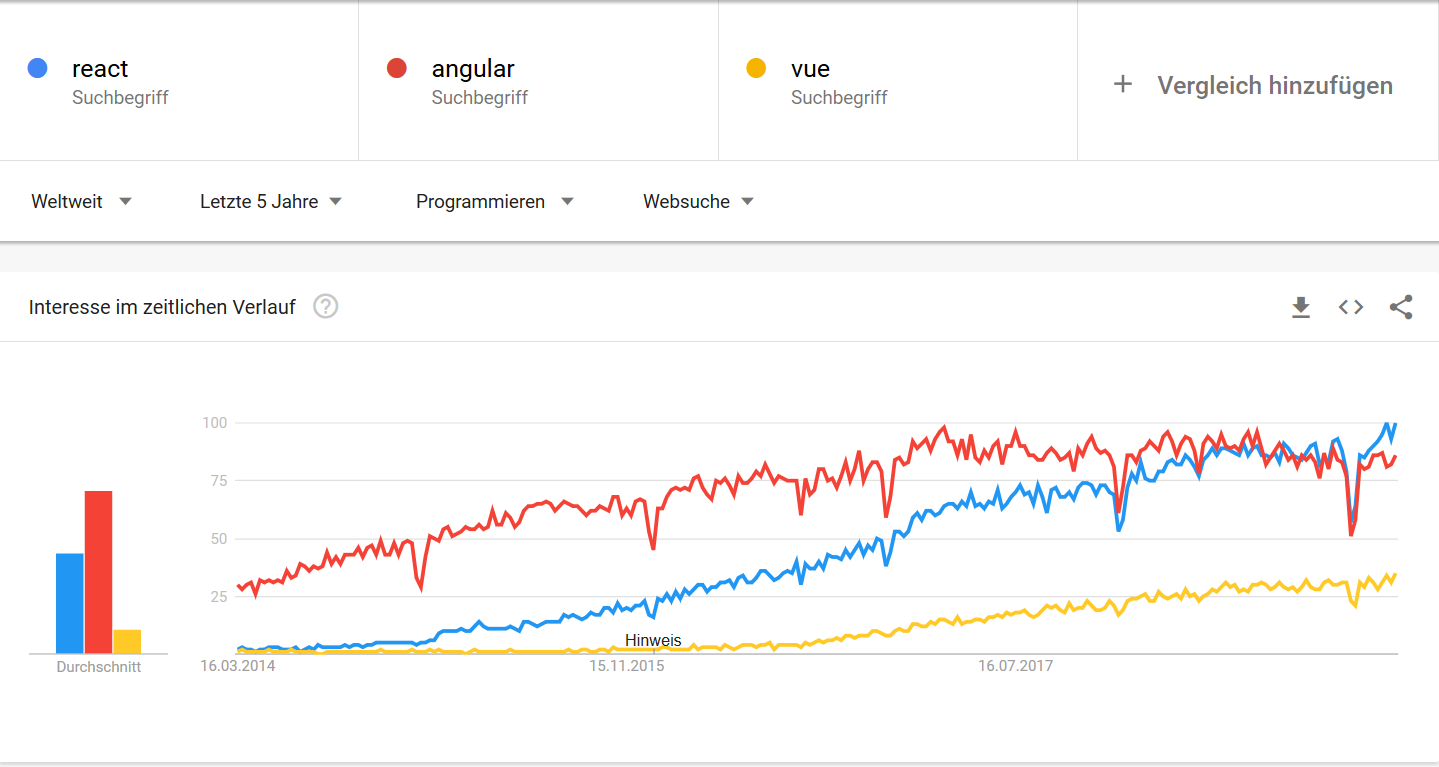
\includegraphics[width=12cm]{../Abbildungen/reactVueAng.png}}
  \caption{Trend der Suchanfragen seit 2014 für React, Angular und Vue \cite{Abb2.8}}
  \label{Trend der Suchanfragen}
\end{figure}
Neben Angular ist Vue Reacts größter Konkurrent. In Abbildung 2.8 ist der Verlauf von Google-Suchanfragen der letzten fünf Jahre, als Indikator der Beliebheit der drei Lösungen, dargestellt. Wie deutlich zu sehen ist, hat React in den letzten Jahren auf Angular aufgeschlossen und es nun sogar überholt. Vue dagegen war lange Zeit kaum bekannt und begann erst in den letzten beiden Jahren aufzuholen.\\\\ 
Vue kann als vielversprechende Alternative zu React gesehen werden. Besonders für Webentwickler die Templates gewohnt sind und sich keine neue Syntax aneignen wollen ist es sehr gut geeignet. In Performanz und Funktionalität ist Vue nahezu gleichwertig zu React und bietet die oben genannten Besonderheiten.
\subsection{Preact}
Preact ist eine sehr kleine Alternative zu React. Die Bibliothek ist nur 3kB groß und damit etwa 15-mal kleiner als React. Preact vereinfacht und entfernt dabei manche Funktionalitäten von React und hat besonders beim Diffing (Feststellen der Änderungen an dem virtuellen DOM) kleinere und schnellere Lösungen \cite{9}. Hinzu kommt, dass in Preact effizientes Recycling von DOM-Elementen betreibt und dadurch zusätzlich Zeit einspart. \\
Die Bibliothek bietet so eine schnellere, kleinere Lösung, besitzt aber weniger Funktionen. Da es derzeit relativ unbekannt ist, sind weit weniger ergänzende Tools für Preact vorhanden. \\\\
Preact kann also besonders für kleine Projekte eine einfachere Alternative zu React darstellen.
\subsection{Riot}
Auch Riot ist, laut dessen Entwicklern, direkt von React inspiriert. Die Bibliothek verfügt aber über eine eigene, knappere Syntax und, wie Preact, über einen vereinfachten Algorithmus für das Diffing. Außerdem sind sowohl ein Routing- als auch ein State-Management-Tool eingebaut. Diese beiden Werkzeuge müssen in React oft noch während dem Projekt implementiert werden.\\
Riot hat nur ein Viertel von Reacts Größe und bietet dennoch große Funktionalität an. Auch diese Lösung ist aber noch relativ unbekannt und weist so langsamere Entwicklung und weniger Tools auf.\\\\
Für Riot gilt daher ähnliches wie für Preact. Besonders für kleine Projekte ist es eine sehr gute Alternative zu React, doch muss es noch an Beliebtheit gewinnen.
\section{Fazit}
React ist eine sehr mächtige und sehr praktische Bibliothek. Die Verbesserungen die es gegenüber früheren Frameworks mit sich brachte waren wegweisend, haben sich durchgesetzt und viele neue Projekte inspiriert. Es bietet zahlreiche Möglichkeiten, Tools und Erweiterungen und kann so jede Anforderung bedienen. Meiner Meinung nach gibt es sogar im Unternehmensbereich wenige Anforderungen denen React nicht gerecht werden kann. \\
Natürlich hat aber auch React, wie oben aufgeführt, Bereiche die verbesserungswürdig sind. Andere Projekte wie Vue, die diese Probleme scheinbar besser gelöst haben, sind bereits auf dem Markt und bieten starke Alternativen. Während React sich momentan dieser großen Beliebheit erfreut, gibt es daher aber auch starke Kritik an der Bibliothek. Bei der großen Geschwindigkeit mit der der Bereich Frontend-Entwicklung wächst, ist es schwer vorauszusagen wie lange React noch so beliebt bleiben wird. \\\\
Diese Sachverhalte führen zu folgender Schlussfolgerung: Momentan ist es definitiv nicht falsch sich für React zu entscheiden. Wie schnell sich das ändert ist aber nicht absehbar. 